    \chapter{Exploitation (future) de la donnée}

En plus de réfléchir à la ou les bases de données à utiliser pour réunir les données, il est également nécessaire de penser à l’utilisation future de la donnée. En effet, il convient de choisir les outils et les interfaces de façon à pouvoir répondre aux besoins des utilisateurs. Dans le cadre du projet sur la formation de l’Europe au XIIème siècle, la future plateforme a pour vocation d’être utilisée spécifiquement dans le cadre de la recherche. Le public visé se compose donc principalement de chercheurs et étudiants. L’enjeu ici est de pouvoir répondre à des questions de recherche.


    \section{Durabilité des technologies}

Nous avons déjà évoqué la question de la durabilité des technologies lors de la présentation des différents types de données permettant le stockage des données. C’est un enjeu important dans le choix des technologies, notamment pour des projets s’étirant sur plusieurs années comme celui du schisme alexandrin.
En effet, certaines technologies peuvent être abandonnées à un temps donné. Pour illustrer ce propos, trois exemples correspondant chacun à un logiciel, un langage et un format de données sont utilisés.


    \subsection{Adobe Flash Player}
    \subsection{Ruby}

\begin{figure}[h]
%centrer l'image
    \centering
    %commande qui permet de charger une image
    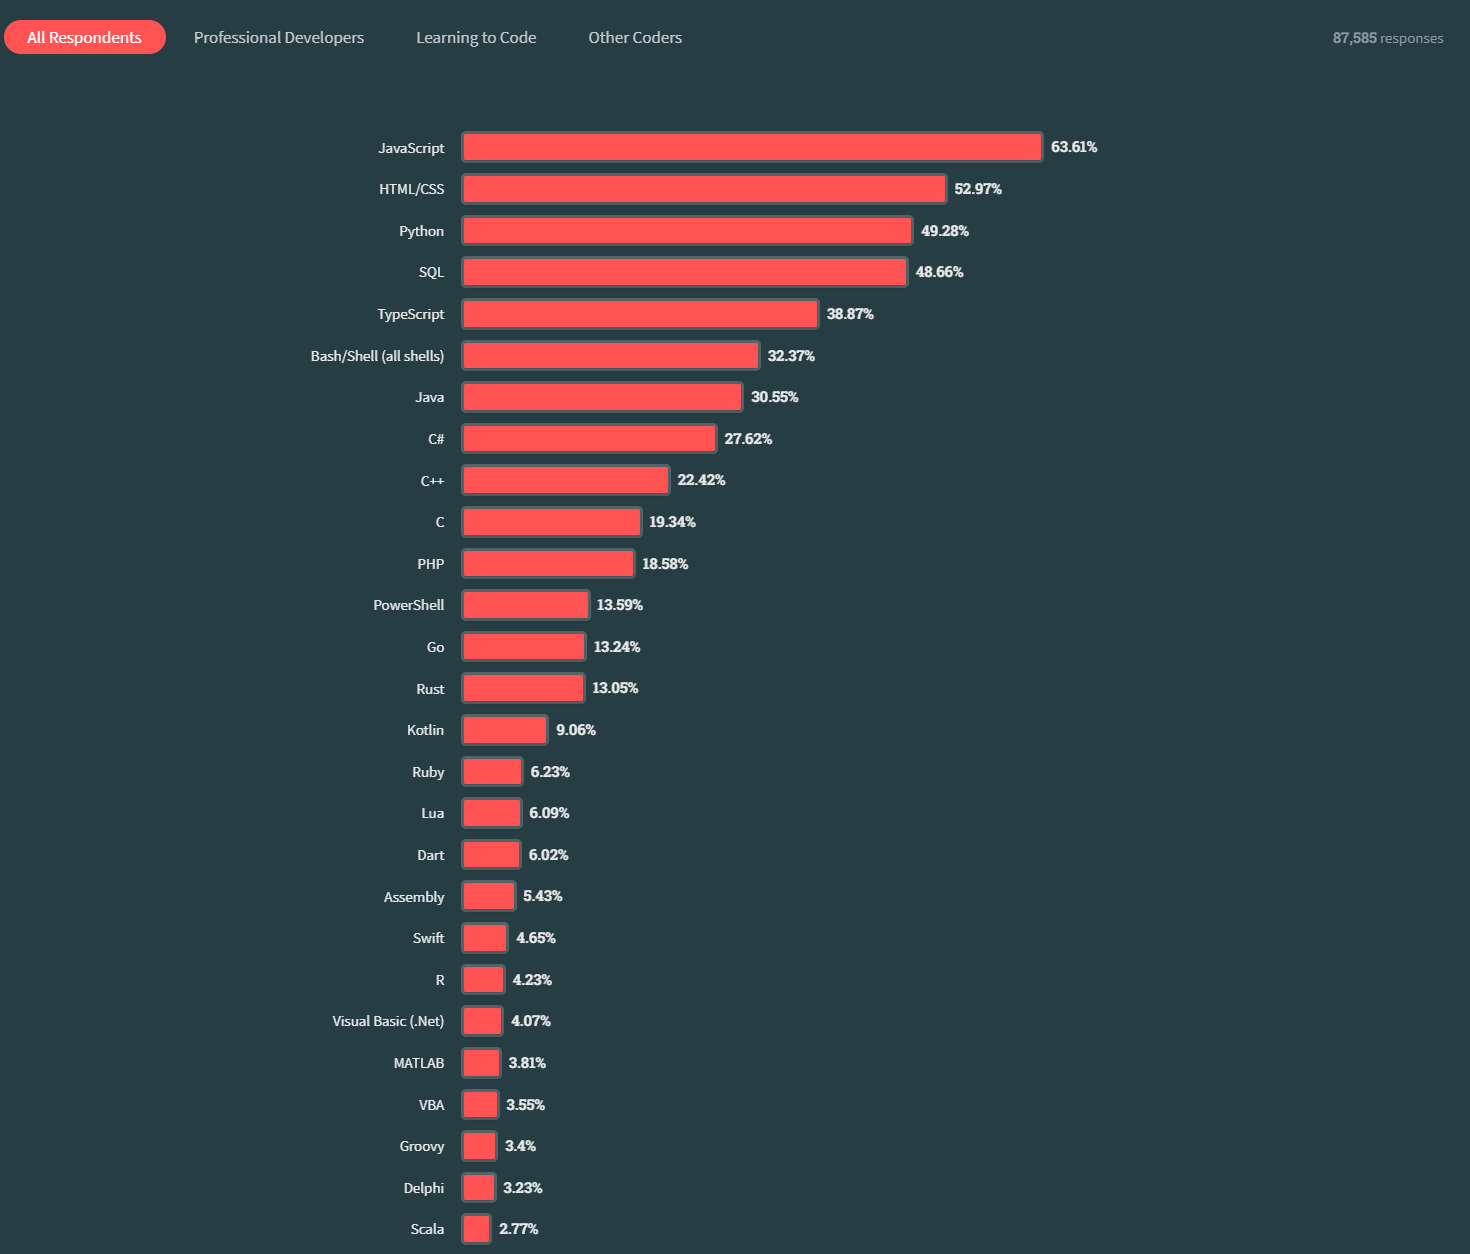
\includegraphics[width=10cm]{images/extrait_sondage_stackoverflow_languages.png}
    %légende
    \caption{Schéma représentant la récupération des données manuellement}
    %label
    \label{fig:schemadonneessauvegarde}
\end{figure}
    
    \subsection{JPEG2000}

JPEG 2000, format présenté en 2000, permet notamment de compresser une image sans perdre la qualité, très utilisé en archives ou en bibliothèques, utilisé à la BnF depuis 2015 pour la numérisation des plans\footnote. Aujourd’hui, plusieurs questions se posent: 
JPEG2000 est supporté que par très peu de navigateur, à des soucis pour s’adapter à l'Open Source et est un format assez complexe\footnote{\textit{Lack of performant open source decoding software}, Open Preservation Foundation, https://wiki.opf-labs.org/display/TR/Lack+of+performant+open+source+decoding+software }. 

En conclusion, concernant les réflexions autour de la durabilité des technologies, tout cela est une question d’arbitrage:
Il est possible d’envisager d’utiliser des logiciels Open Source pour éviter le coût financier. De plus, il est plus probable que les technologies open source soient reprises par la communauté.
Possibilité d’estimer la pérennité d’une technologie en fonction de la taille de la communauté. Par exemple, le XML TEI est une grande communauté, notamment avec les guidelines et le TEI consortium, ce qui en fait, comme dit plus haut, un langage pérenne et un choix sûr. Pareil pour le SQL, qui existe depuis presque 50 ans\\
Le coût des technologies est aussi un critère à prendre en compte, surtout dans le cadre d’un projet aussi long. Maintenance importante aussi quand on utilise des logiciels de niche. \\

Le choix des technologies à utiliser dans un projet devient très vite un casse-tête, car il faut pouvoir à la fois choisir des logiciels et des langages accessibles aux chercheurs qui n’ont pas spécialement de formation en informatique tout en répondant aux besoins très spécifiques du projet.



    \section{Faire le lien entre les chercheur.se.s et la donnée: UX/UI}
    \subsection{Interfaces graphiques et outils}
    \subsection{Formats de données}
    
    \section{Favoriser la collaboration et l'échange}
    \subsection{API et interopérabilité}
    \subsection{Open Data}